\begin{figure}
\centering
    
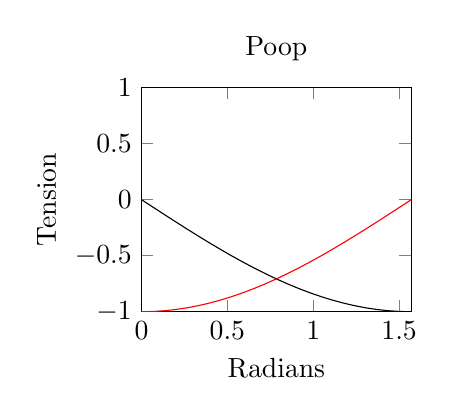
\begin{tikzpicture}
\begin{axis}[
    title=Poop,
    xlabel={Radians},
    ylabel={Tension},
    ymin=-1, ymax=1,
    xmin=0, xmax=pi/2,
    scale=0.5,
]
    \addplot [domain=0:pi/2] {-sin(deg(x))};
    \addplot [red, domain=0:pi/2] {-cos(deg(x))};
\end{axis}
\end{tikzpicture}


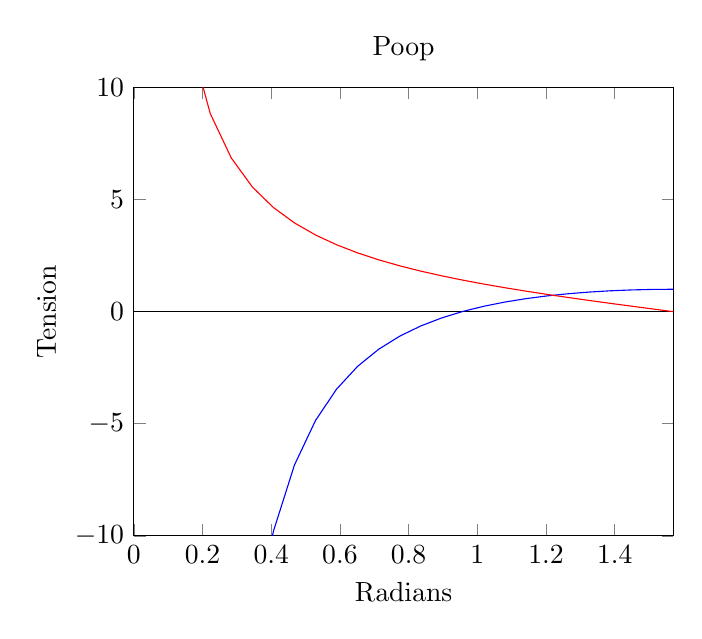
\begin{tikzpicture}
\begin{axis}[
    title=Poop,
    xlabel={Radians},
    ylabel={Tension},
    ymin=-10, ymax=10,
    xmin=0, xmax=pi/2
]
    \addplot [domain=0:pi/2] {0};
    \addplot [blue, domain=0.1:pi/2] {1-2*cot(deg(x))^2};
    \addplot [red, domain=0.1:pi/2] {2*cot(deg(x))};
\end{axis}
\end{tikzpicture}

\begin{tikzpicture}
\begin{axis}[
    title=Poop,
    xlabel={$\Gamma$},
    ylabel={F/M},
    ymin=-10, ymax=10,
    xmin=0, xmax=90, xtick={0,90}, xticklabel=$\pgfmathprintnumber{\tick}^\circ$,
]
    \addplot [domain=0:90, dashed] {0};
    \addplot [domain=1:90, samples=100] {-cot(x)};
\end{axis}
\end{tikzpicture}

\end{figure}

\begin{figure}
\centering

\begin{tikzpicture}
\begin{axis}[
    title=Poop,
    xlabel={$\Gamma$},
    ylabel={F/M},
    ymin=-10, ymax=10,
    xmin=0, xmax=90, xtick={0,54.7,90}, xticklabel=$\pgfmathprintnumber{\tick}^\circ$,
]
    \addplot [domain=0:90, dashed] {0};
    \addplot [domain=1:90, samples=100] {(1-2*cot(x)^2) / (2*cot(x))};
    \addplot [mark=none, dashed] coordinates {(54.7,-10) (54.7,10)};
\end{axis}
\end{tikzpicture}

\begin{tikzpicture}
	\begin{polaraxis} [
	legend style={at={(axis cs:35,3.5)},anchor=south west, draw=none},
	xmin=0, xmax=90, xtick={0,90}, xticklabel=$\pgfmathprintnumber{\tick}^\circ$,
	ymin=0, ymax=3, ytick={1,2},
	]
	\addplot+[mark=none, domain=0:90, samples=100] {abs(-cot(x))};
	\addlegendentry{$\left|\frac{T_x}{T_y} \right|$};
%	\addplot+[mark=none, dashed] coordinates {(0,0) (54.7,3)};
	\end{polaraxis}
\end{tikzpicture}

\begin{tikzpicture}
	\begin{polaraxis} [
	    legend style={at={(axis cs:35,3.5)},anchor=south west, draw=none},
	    xmin=0, xmax=90, xtick={0,54.7,90}, xticklabel=$\pgfmathprintnumber{\tick}^\circ$,
	    ymin=0, ymax=3, ytick={1,2},
	    ]
	\addplot+[mark=none, domain=0:90, samples=100] {abs((1-2*cot(x)^2)/(2*cot(x)))};
	\addlegendentry{$\left|\frac{F}{M} \right|$};
	\addplot+[mark=none, dashed] coordinates {(0,0) (54.7,3)};
	\end{polaraxis}
\end{tikzpicture}

    
\caption{Caption}
\label{fig:my_label}
\end{figure}